\lecture{8}{2025-03-12}{Prediction, learning, and Cross-Entropy-Loss}{}

\begin{parag}{Billard Balls}
    Can we use the 20 questions approach to solve the 14 bullars riddle?
    \begin{subparag}{Answer}
        No, because the kind of questions that we can "ask", when wa are weighing, is quite limited.\\
        For instance, the first question cannot be "is $1$ or $2$ heavy?".
        
    \end{subparag}

\end{parag}
\begin{parag}{Strategies}
    But is there a strategy that requires only $3$ weighings?
    \\
    From source compression, we can establish the following facts?
    \begin{itemize}
        \item For each weighings, the three outcomes must be equally likely
        \item The weighings must be independent of each other
    \end{itemize}
    \begin{framedremark}
        It is because we carefully selected the numbers (alphabet size of 27; each weighing has $3$ possible outcomes) that there is a strategy that exactly matches the entropy lower bound $3$ weighings. If you change the numbers, it will not generally be true that there is a strategy that \textit{exactly} matches the lower bound.
    \end{framedremark}
\end{parag}
\subsection{Prediction, Learning and cross-Entropy Loss}
The goal here is to change the way to use entropy, entropy has always be seen as something that \textit{means} something, a lower bound, a quantity of information. Here we will use it to do calculation juste like a \textit{tool}.
\begin{parag}{Example}
\begin{center}
    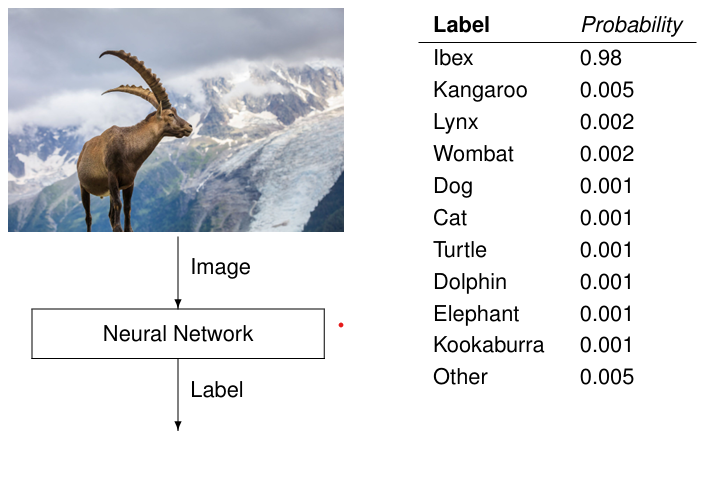
\includegraphics[scale=0.6]{12025-03-12.png}
\end{center}
\begin{framedremark}
    There weren't probability at this time in the slide so imagine without it
\end{framedremark}

The question we want to ask is, \textit{"Is our neural network performing well"}\\
\begin{itemize}
    \item Given an image $ \mathcal{X}$
    \item Our machine (Neural network)
    \item Outputs $Q(x)$
    \item The label: Label$(x)$
\end{itemize}
\begin{subparag}{Zero-one loss}
    \begin{align*}
        L\{Q(x) \neq \text{Label}(x)\}\\
        = \begin{cases}
            1 \text{ if } Q(x) \neq \text{Label}(x)\\
            0 \text{ if } Q(x) = \text{Label}(x)
        \end{cases}
    \end{align*}
    Given a lot of image, we want to have a \important{Classification error}:
    \begin{align*}
        \frac{\sum_{ \mathcal{X}} L\{Q(x) \neq \text{Label}(x)\}
}{ \text{number of images}}
    \end{align*}
    Is the function of mis-labeled images.
\end{subparag}
\begin{subparag}{Pros and Cons}
    \textbf{Pros}
    \begin{itemize}
        \item Very intuitive
        \item Interpretable
    \end{itemize}
    \textbf{Cons}
    \begin{itemize}
        \item Not differentiable
    \end{itemize}
\end{subparag}
\begin{subparag}{With probability}
    Our neural network produces:
    \begin{align*}
        Q( \text{label} \mid \text{image})
    \end{align*}
    The true label distribution is:
    \begin{align*}
        P_{true}( \text{label} \mid \text{image}) = \begin{cases}
            1, \text{ correct label}\\
            0, \text{ wrong label}
        \end{cases}
    \end{align*}
    (We are assuming for simplicity that for each image, there is a single correct label).\\
    \begin{itemize}
        \item Ideally, we would like:
            \begin{align*}
                Q( \text{label} \mid \text{image}) = P_{true}( \text{label} \mid \text{image}) \; \; \forall \text{pairs}
            \end{align*}
    \end{itemize}
   However this is only a dream
   \begin{itemize}
       \item Instead, people like to consider \important{cross entropy loss}
       \item that is, we wish ou $Q($label$ \mid $image) to \important{minimize}
           \begin{align*}
               L(P_{true}( \text{label} \mid \text{image}), Q( \text{label} \mid \text{image}) \\
               = - \sum_{ \text{label}}P_{true}( \text{label} \mid  \text{image})\log_D Q( \text{label} \mid \text{image})
           \end{align*}
       \item Given training data (image, label), for $i = 1, 2, \dots, n$ we select $Q($ label $ \mid $ image) to minimize the cross entropy loss.
   \end{itemize}
    
\end{subparag}
\end{parag}
\begin{parag}{Cross entropy loss}
    \begin{align*}
        L(P, Q) = -\sum_y P(y)\log_DQ(y)
    \end{align*}
    Where
    \begin{itemize}
        \item $P$ is the true distribution
        \item $Q$ is our approximation (via neural network)
    \end{itemize}
    Why is it popular?
    \begin{itemize}
        \item Good properties for training with "gradient descent" in certain standard architectures.
        \item Theoretical properties.
    \end{itemize}
\end{parag}

\begin{parag}{A (very) simple neural network}

Takes a screen of the blackboard
\begin{itemize}
    \item it transform the image into a vector
    \item Then takes is through the weighs $w_i$ all the way to $d$
       \item the we take it through the soft max which is two functions:
           \begin{align*}
               Q(o \mid  x) &= \frac{e^{z_0}}{e^{z_0} + e^{z_1}} \\
               Q(1 \mid  x) &= \frac{e^{z_1}}{e^{z_0} + e^{z_1}}
           \end{align*}
\end{itemize}
The goal is given a lot of training data, we want to select the $w_0, b_0, w_1, b_1$ such at to minimize the total cross entropy loss.
\end{parag}
\begin{parag}{For a single image $ \mathcal{X}$}
    because why is juste binary we use:
    \begin{align*}
        L(P(y \mid  x), Q(y \mid  x)) \\
        &= - \sum_y P(y \mid  x) \log Q(y \mid  x)\\
        Q(o \mid  x) = \frac{e^{z_0}}{e^{z_0} + e^{z_1}} = \frac{e^{x \cdotw_0 + b_0}}{e^{X \cdot w_0 + b_0} + e^{X \cdot w_1 + b_2}}\\
        &= \begin{cases}
            \log \frac{e^{x \cdot }{}
       \end{cases}

    \end{align*}
    \textbf{Total Loss}
    \begin{align*}
        L_{total}(w_o, b_o, w_1, b_1) = -\sum_{i = 1}^k\log \frac{e^{x_iw_0 + b_0}}{e^{x_iw_0 + b_0} + e^{x_i \cdot w_1 + b_1}} - \sum_{i = k+1}^n \log \frac{e^{w_1k_i + b_1}}{e^{w_0x_i + b_0} + e^{w_1x_i + b_1}}
    \end{align*}
    

\end{parag}
\begin{parag}{Cross entropy loss}
    Cross entropy loss:
    \begin{align*}
        L(P, Q) = - \sum_y P(y)\log_DQ(y)
    \end{align*}
    \begin{theoreme}
        For a fixed probability distribution $P$, the minimum:
        \begin{align*}
            \text{min}_QL(P, Q)
        \end{align*}
        Is attained if and only if we selected $Q^* = P$ in this case, 
        \begin{align*}
            L(P, Q^*) = L(P, P) = H(P)
        \end{align*}
        Where $H(P)$ is the entropy of the probability distribution $P$
    \end{theoreme}
    
    
    \begin{subparag}{Proof}
        The proof, which will be done in class, uses once again the "IT inequality".\\
        The theorem is saying this:
        \begin{align*}
            H(P) \leq L(P, Q)
        \end{align*}
        With equality in one case which is $P = Q$.
        \begin{align*}
            H(P) - L(P, Q) &\leq 0 \\
            -\sum_yP(y)\log P(y) + \sum_y P(y) \log Q(y) &\leq 0 \\
            = sum_yP(y)\log \frac{Q(y)}{P(y)} \leq \sum_yP(y) \left[ \frac{Q(y)}{P(y)} - 1 \right]\log (e) \\
            = \sum_y(Q(y) - P(y)) \log (e) \\
            = 0
        \end{align*}
        
    \end{subparag}

    \begin{subparag}{Note}
        We don't see it in AICC II but let's introduce the notion: \important{KL-Divergence} (aka KL distance):
        \begin{formule}
            \begin{align*}
                D_{kl}(p \mid  \mid k) = \sum_y p(y)\log \frac{P(y)}{Q(y)}
            \end{align*}
  \begin{itemize}
      \item Fact 1: \\
          $D_{kl}(P \mid \mid Q) \geq 0$ with equality iff $P = Q$ (this is just the proof seen earlier
  \end{itemize}          
            
        \end{formule}
    \end{subparag}
\end{parag}

    \section{Summary of chapter 1}
    \begin{parag}{Entropy}
        \begin{align*}
            H_D(X) = - \sum_x p(x)\log_D p(x)
        \end{align*}
        For $D = 2$, we simply write $H(X)$ and we all the units bits.\\
        Entropy has many useful properties, including:
        \begin{itemize}
            \item $0 \leq H_D(X) \leq \log_D \mid \mathcal{X} \mid$
            \item $H_D(X \mid  Y) \leq H_D( X)$ with equality if and only if $X$ and $Y$ are independent
            \item $H_D(X, Y) = H_D(X) + H_D(Y \mid  X)$
        \end{itemize}
        
    \end{parag}
    \begin{parag}{Data Compression}
        \begin{itemize}
            \item Every uniquely decodable binary code must use at least $H(X)$ bits per symbol on average
            \item There exists a binary code that uses between $H(X)$ and $H(X) + 1$ bits per symbol on average
            \item Hence, for a source string of length $n$:
                \begin{itemize}
                    \item Every uniquely decodable binary code must use at least $H(S_1, S_2, $
                \end{itemize}
        \end{itemize}
    
    \end{parag}
   \begin{parag}{Models}
   \begin{subparag}{Coin Flip}
       The coin flip is not convertible, With a file of result, there is no way to compress the file
   \end{subparag}
   \begin{subparag}{Sunny Rainy}
       Here, the entropy, is not $1$ then we are able to compress the file here.\\
       This is the first view of mark of model.\\
       Given $S_1, S_2, S_3, \dots$, Are $S_1, S_3$ independent?
       \\
       \begin{align*}
           p(S_1, S_3) &= \sum_{S_2} p(S_1, S_2, S_3)\\
                       &= \sum_{S_2}p(S_1)p(S_2 \mid S_1)p(S_3 \mid S_2) 
       \end{align*}
       
   \end{subparag}
   \end{parag}
 \begin{parag}{Entropy and algorithm}
     We explored examples where entropy can give a lower bound on algorithmic performance.
     \begin{itemize}
         \item Example: in search-type problems, give a lower bound on the minimum number of necessary queries.
     \end{itemize}
 
 \end{parag}
    
 \begin{parag}{Cross-Entropy Loss}
     \begin{itemize}
         \item Machine (e.g., Neural Network) outputs a distribution $Q(y)$ over all possible labels
         \item Cross entropy loss: Select $Q(y)$ to minimize:
             \begin{align*}
                 L(P, Q) = - \sum_y P(y)\log_DQ(y)
             \end{align*}
             
     \end{itemize}
 
 \end{parag}
 
    
